\subsection{Segmentering med eksempelbilleder}
Som vi har nævnt i tidligere afsnit, har vi opnået de bedste resultater ved at lede efter vesiklerne selv, i stedet for at lede efter egenskaber som kanter og andet. Vi forsøger derfor at detektere vesiklerne ved at folde med billeder af disse. Vi laver en liste af vesikler der skal repræsentere mangfoldigheden af vesikler. Da der er forskel på vesiklernes intensitetsværdier, form og størrelse er det nødvendigt med denne liste af vesikler, i stedet for bare at nøjes med en enkelt. Vi tager så hver enkelt vesikel og folder med billedet. For hver pixel i billedet vælger vi et udsnit på størrelse med vesiklen der har centrum i den pixel vi er gået ud fra. Vi benytter en funktionen \texttt{nlfilter} i MATLAB til at flytte udsnittet rundt på billedet. Funktionen tilføjer 0'er i de pixels i udsnittet der går udover kanten af billedet.

Ideen er at der for hvert udsnit udregnes en værdi der svarer til den euklidiske afstand til vesiklen der foldes med,
\begin{align}
	\sum_m\sum_n\left(I_{ij}(m,n)-J(m,n)\right)^2\label{ali:postmethod_conv_pre1}
\end{align}
hvor $I_{ij}$ er udsnittet af billedet med centrum i $(i,j)$ og $J$ er det vesikelbillede vi folder med. 

Dette er stærkt relateret til en foldning fordi hvis vi ser på $I_{ij}$ og $J$ som vektorer i stedet for matricer, kan vi omskrive (\ref{ali:postmethod_conv_pre1}) til
\begin{align}
	||\vec{I}-\vec{J}||^2 = (\vec{I}-\vec{J})^T(\vec{I}-\vec{J}) = \vec{I}^T\vec{I} + \vec{J}^T\vec{J}-2\vec{I}^T\vec{J}
\end{align}
Ser vi så på det sidste led, $2\vec{I}^T\vec{J}$, er dette jo netop lig $\sum_m\sum_nI_{ij}(m,n)J(m,n)$, som kan omskrives til foldningen $I*J(i,j)$. Dette betyder at vores formel er en foldning med en lokal normering. For at lette læsningen vil vi blot henvise til dette som en afstand. Vi vælger at benytte den euklidiske afstand i stedet for udelukkende at folde med vesiklen for at slippe for problemer i mørke områder. Hvis $I_{ij}$ er et udsnit med 0'er i alle indgange, vil $I*J(i,j)=\sum_m\sum_nI_{ij}(m,n)J(m,n)=0$. Da værdier gående imod 0 er hvad vi er ude efter, er dette ikke godt, og altså grunden til at vi benytter euklidisk afstand i stedet.

For at normalisere skalaerne trækker vi middelværdien fra hver indgang i udsnittene, og dividerer med standardafvigelsen, som vi så gemmer i centerpixlen. Udregningen af værdierne i hver pixel gøres med ligningen

\begin{align}
	\sum_m\sum_n \left(\frac{I_{ij}-mean(I_{ij})}{std(I_{ij})}-\frac{J-mean(J)}{std(J)}\right)^2 \label{ali:postmethod_conv}
\end{align}

Funktionen tager altså et område på samme størrelse som den eftersøgte vesikel, normerer hver indgang i dem begge for at de er på samme skala, trækker dem fra hinanden og kvadrerer resultatet. Summen af dette er så den euklidiske afstand mellem de to områder.

Det resulterende billede indeholder så fra 0 og opefter. Hvis et udsnit ligner den vesikel der søges, vil $I_{ij}$ og $J$ i (\ref{ali:postmethod_conv}) jo være næsten ens, sumfunktionen vil altså gå imod 0 alt efter hvor godt området ligner. Omvendt vil sumfunktionen give høje værdier hvis området ikke ligner den eftersøgte vesikel. Da høje værdier er lig med hvid, og værdier mod 0 er lig med sort, vil det resulterende billede altså have mørke områder hvor der er fundet vesikler. 

Et eksempel på et område vi ønsker at finde vesikler i, og en vesikel vi finder afstand med, ses i figur \ref{fig:postmethod_conv_pre}. I figur \ref{fig:postmethod_conv_area1} ses det område hvor cellen er.

\begin{figure}[H]
		\centering
		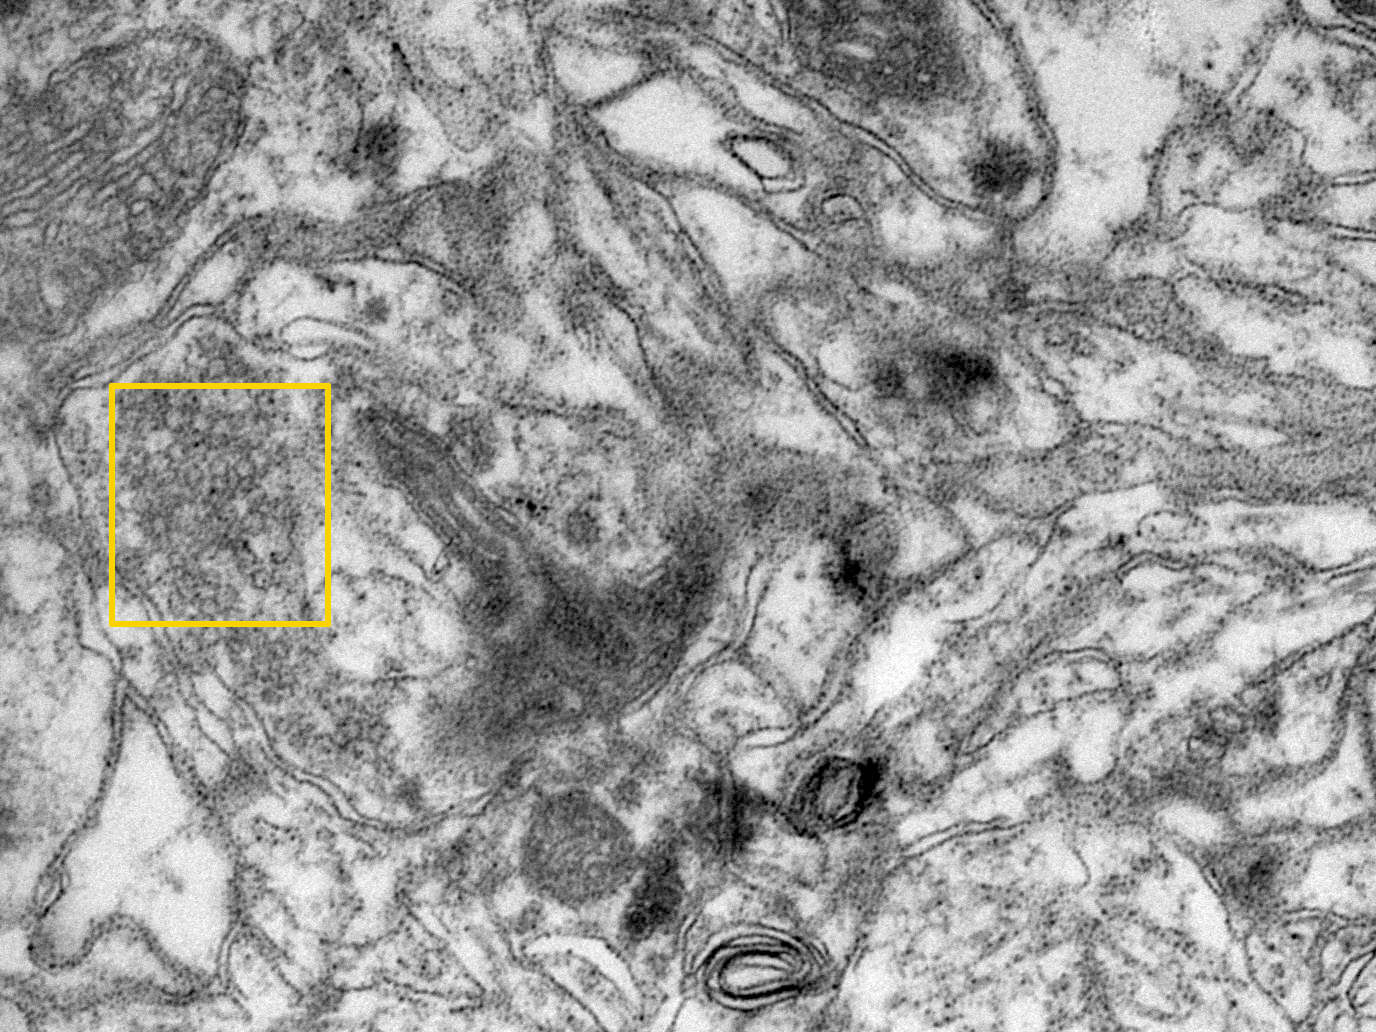
\includegraphics[scale=0.5]{files/postmethod/img/area_1.png}
	\caption{Billede med cellen vi vil undersøge markeret.\label{fig:postmethod_conv_area1}}
\end{figure}

\begin{figure}[H]
	\begin{minipage}[b]{0.5\linewidth}
		\centering
		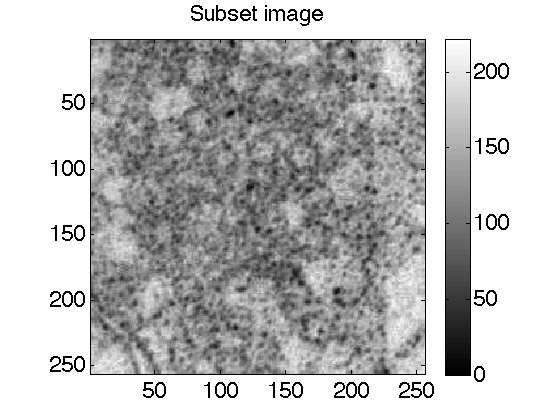
\includegraphics[scale=0.5]{files/postmethod/img/conv_1.png}
	\end{minipage}
	\hspace{0.5cm}
	\begin{minipage}[b]{0.5\linewidth}
		\centering
		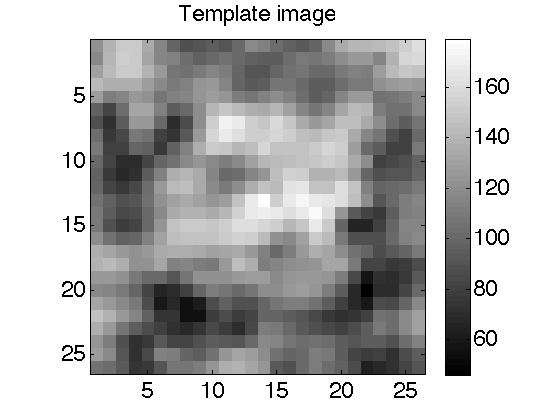
\includegraphics[scale=0.5]{files/postmethod/img/conv_2.png}
	\end{minipage}
	\caption{Til venstre ses en celle hvor vi ønsker at detektere vesikler. Til højre ses den vesikel der ledes efter.\label{fig:postmethod_conv_pre}}
\end{figure}

Vi har i det samme billede også markeret ground truth, som vi i det følgende måler vores resultater ud fra. Der er i billedet markeret 9 områder hvor der er en vesikel. I virkeligheden er der 10, men da det sidste område ligger tæt på kanten har vi valgt ikke at tælle dette med, ligesom vi så heller ikke tæller andre områder som algoritmen finder nær kanten med. Dette er naturligvis fordi vi ikke kan stole på de resultater vi får nær kanten, da \texttt{nlfilteret} som vi benytter bare udfylder manglende pixels med 0'er. Ground truth-billedet ses i figur \ref{fig:postmethod_conv_gt}. 

\begin{figure}[H]
		\centering
		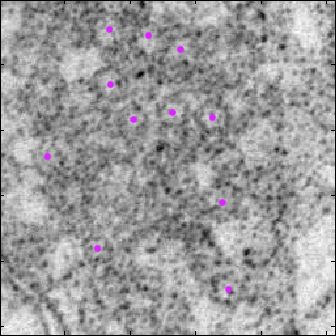
\includegraphics[scale=0.65]{files/postmethod/img/ground_truth.png}
	\caption{Ground truth markeret med pinke prikker i det originale billede.\label{fig:postmethod_conv_gt}}
\end{figure}

Som beskrevet bygger vores algoritme et nyt billede på samme størrelse med det originale. Dette nye billede kalder vi et \texttt{Distance Map}, da hver indgang består af afstanden til den vesikel der er blevet foldet med. Et eksempel på et sådant billede ses til venstre i figur \ref{fig:postmethod_conv_post}. Til højre ses det samme billede, hvor en tærskelværdi på 35\% har markeret de mørkeste pixelværdier med hvidt i det sorte canvas.

\begin{figure}[H]
	\begin{minipage}[b]{0.5\linewidth}
		\centering
		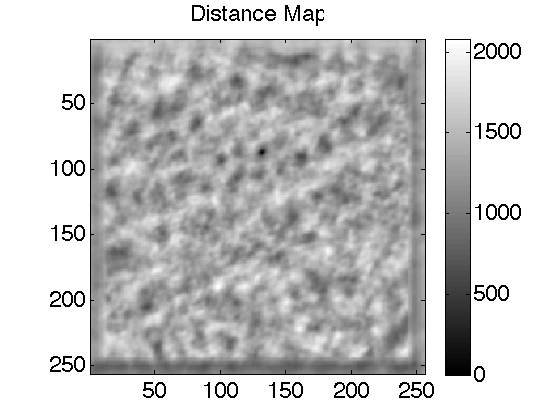
\includegraphics[scale=0.5]{files/postmethod/img/conv_3.png}
	\end{minipage}
	\hspace{0.5cm}
	\begin{minipage}[b]{0.5\linewidth}
		\centering
		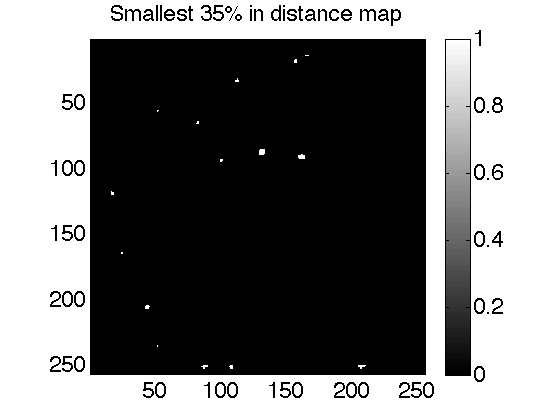
\includegraphics[scale=0.5]{files/postmethod/img/conv_4.png}
	\end{minipage}
	\caption{Til venstre ses det resulterende distance map. Til højre ses samme billede efter en tærskelværdi på nederste 35\% af farveværdierne.\label{fig:postmethod_conv_post}}
\end{figure}

For lettere at se markeringen af vesiklerne har vi plottet de fundne områder med farver i det originale billede på figur \ref{fig:postmethod_conv_photoshop}. De grønne områder er de vesikler som funktionen korrekt har markeret, altså sande positive. De blå områder er hvor funktionen ikke har markeret nogen vesikler selvom de i virkeligheden er der, altså falske negative. Til sidst er der områderne markeret med rødt. Dette er områder som funktionen har markeret som vesikler selvom der ikke er nogen, altså falske positive. Dette betyder altså at ground truth i billedet er de grønne samt i blå.

I eksemplet her er der altså fundet 5 sande positive, 6 falske negative og 6 falske positive. Dette giver en sand-positiv-ratio, også kaldet sensitivity \cite{roc:sensitivity}, på
\begin{align}
	SPR = \frac{SP}{SP+FN} = \frac{5}{11} = 0.455
\end{align}
og antallet af fejldetekterede vesikler (fejl-ratio) er
\begin{align}
	FR = \frac{FP}{FP+SP} = \frac{6}{11} = 0.545
\end{align}

\begin{figure}[H]
		\centering
		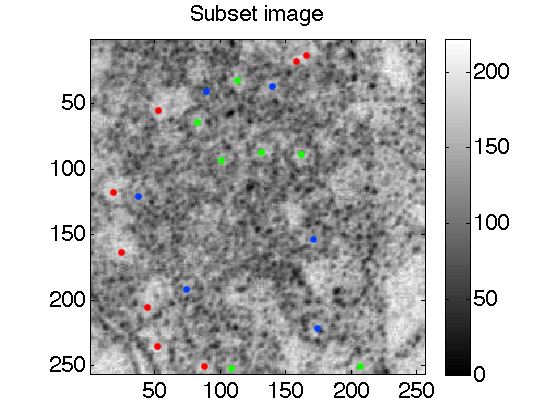
\includegraphics[scale=0.65]{files/postmethod/img/conv_5.png}
	\caption{Oprindelige billede med markerede områder. Grønne er korrekt detekterede vesikler. Røde er forkert detekterede vesikler. Blå er vesikler der ikke blev detekteret.\label{fig:postmethod_conv_photoshop}}
\end{figure}

Som det ses på billedet er der både flere falske positive og falske negative. Resultatet er dog efter en foldning med en enkelt vesikel. Vi kan derfor vælge at regulere tærskelværdien for hvor tæt de fundne områder skal være på 0. At hæve tærskelværdien kan medføre at vi finder flere vesikler, men også flere falske positive, hvorimod at sænke tærskelværdien kan reducere antallet af falske positive, men kan dog også fjerne et antal af de sande positive. I forhold til vores nuværende eksempel kan vi prøve at se på hvordan tærskelværdien ligger. Ser vi f.eks. på området omkring den korrekt fundne vesikel i nedre højre hjørne, kan vi plotte værdierne omkring denne. Dette har vi gjort i figur \ref{fig:postmethod_conv_lines_1}, hvor vi også har tegnet en linje ud fra 700 på y-aksen, der ca. svarer til 35\%, da dette er vores nuværende tærskelværdi. Vi ved fra ground truth at der i dette område ikke er flere vesikler, hvorfor at vi kan se at vi ikke skal hæve tærskelværdien til mere end ca. 780 før at der vælges flere falske positive. 

\begin{figure}[H]
		\centering
		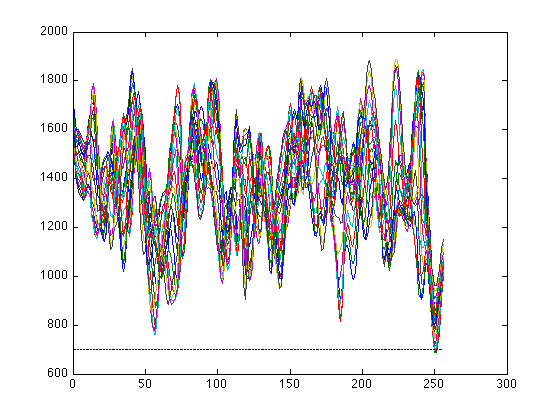
\includegraphics[scale=0.9]{files/postmethod/img/conv_lines_1.png}
	\caption{Udsnit af distance mappet omkring korrekt detekteret vesikel. Hver tegnet linje svarer til en søjle i distance mappet. Ud ad x-aksen er hvert punkt, og op ad y-aksen er afstanden til den søgte vesikel i den indgang i mappet. Tærskelværdien 700 markeret.\label{fig:postmethod_conv_lines_1}}
\end{figure}
% HEDDER DET AF ELLER AD I OVENSTÅENDE CAPTION?

Omvendt har vi i figur \ref{fig:postmethod_conv_lines_2} plottet området omkring to falske positive vesikler. Her kan vi aflæse at vi ved at sænke tærskelværdien til f.eks. 600 ville slippe af med disse. Går vi så tilbage og ser på figur \ref{fig:postmethod_conv_lines_1} ser vi dog at dette vil medføre at den korrekt detekterede vesikel ikke vil blive detekteret.

\begin{figure}[H]
		\centering
		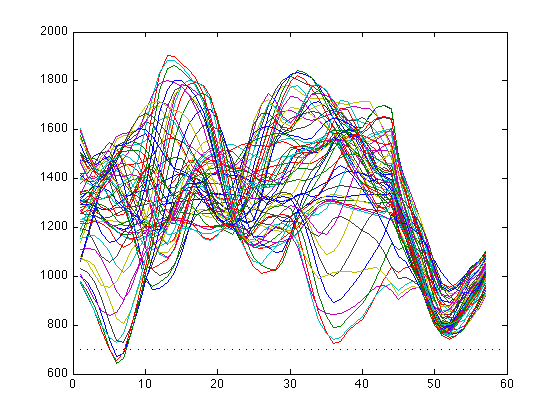
\includegraphics[scale=0.9]{files/postmethod/img/conv_lines_2.png}
	\caption{Udsnit af distance mappet omkring korrekt detekteret vesikel. Hver tegnet linje svarer til en søjle i distance mappet. Ud ad x-aksen er hvert punkt, og op ad y-aksen er afstanden til den søgte vesikel i den indgang i mappet. Tærskelværdien 700 markeret.\label{fig:postmethod_conv_lines_2}}
\end{figure}

Da vores algoritme finder afstande til en liste af vesikler er vi dog mere interesserede i at den finder færre vesikler, mod at den holder antallet af falske positive nede. Vores mål er da at tage de fundne vesikler efter hver foldning, og kombinere til et endeligt resultat. I nedenstående tabel ses vores resultater efter forsøg med forskellige tærskelværdier og forskellige  vesikler. Alle vesiklerne er fra billedet som der efterfølgende findes afstande til. Vi viser kun de resultater der har fundet andre vesikler end den der foldes med. I SPR og FR søjlerne har vi markeret de bedste værdier for hver vesikel.
\begin{table}[H]
	\centering
\begin{tabular}{l|l|l|l|l|l|l|l}
	$\#$ & Vesikel & Tærskelværdi i $\%$ & SP & FP & FN & SPR & FR \\\hline
	1	&	A	&	0.30	& 2		& 0		&9 	&0.182 			&\textbf{0}\\\hline
	2	&	A	&	0.31	& 2		& 1		&9 	&0.182 			&0.333\\\hline
	3	&	A	&	0.32	& 4		& 1		&7  &0.364 			&0.2\\\hline
	4	&	A	&	0.33	& 4		& 1		&7  &0.364 			&0.2\\\hline
	5	&	A	&	0.34	& 5		& 3		&6  &\textbf{0.455}	&0.375\\\hline
	6	&	A	&	0.35	& 5		& 6		&6  &0.455 			&0.545\\\hline
	7	&	A	&	0.36	& 5		& 8		&6  &0.455			&0.615\\\hline	
	8	&	B	&	0.38	& 2		& 7		&9 	&\textbf{0.182}	&\textbf{0.778}\\\hline
	9	&	B	&	0.39	& 2		& 9		&9 	&0.182 			&0.818\\\hline
	10	&	B	&	0.40	& 2		& 12	&9 	&0.182 			&0.857\\\hline	
	11	&	C	&	0.33	& 3		& 7		&8 	&0.273 			&0.7\\\hline
	12	&	C	&	0.34	& 5		& 8		&6 	&\textbf{0.455}	&\textbf{0.615}\\\hline
	13	&	C	&	0.35	& 5		& 12	&6 	&0.455 			&0.706
\end{tabular}
\caption{Tabel over forskellige tærskelværdiers påvirken på SPR og FR for 3 forskellige vesikler.\label{tab:postmethod_tabelll}}
\end{table}

Hver af ovenstående vesikler (A, B og C) er et udsnit af det originale billede, kun indeholdende området for en enkelt vesikel, ligesom vist til højre i figur \ref{fig:postmethod_conv_pre}. Af ovenstående kan vi altså aflæse at vesikel A er bedst med en tærskelværdi på 30\% hvis vi går efter at minimere antallet af falske positive, og 34\% hvis vi går efter at maksimere vores sand-positv-ratio. Vesikel B er bedst ved 38\% og til slut er vesikel C bedst ved 34\%. Vi prøver derfor at sammensætte det kombinerede billede detektion med vesikel A og C, først med tærskelværdi på 30\% og dernæst på 34\%. 
% Forhold mellem SPR / FR diskuteres her?

Vores første resultat ses til venstre i figur \ref{fig:postmethod_conv_ves_1}. Dette er det kombinerede billede med vesikel A og C og tærskelværdi på 30, hvor vi igen har markeret korrekt detekterede vesikler med grøn, forkert detekterede med rød og falske negative med blå. Vi udregner så vores sand-positiv-ratio og fejl-ratio igen.

\begin{align}
	SPR &= \frac{SP}{SP+FN} = \frac{3}{11} = 0.273\\
	FR &= \frac{FP}{FP+SP} = \frac{2}{5} = 0.4
\end{align}
Her kan vi aflæse at vi ved at ligge resultatet fra foldningen med vesikel C oveni vesikel A's resultat, har vi hævet vores sand-positiv-ratio fra 0.182 til 0.273. Vi har samtidig hævet vores fejl-ratio fra 0 til 0.4, da der findes 2 falske positive mod 0 før.  

Vores andet resultat hvor vi har benyttet tærskelværdi på 34\% ses til højre i figur \ref{fig:postmethod_conv_ves_1}. Her udregner vi også vores ratioer igen.

\begin{align}
	SPR &= \frac{SP}{SP+FN} = \frac{8}{11} = 0.727\\
	FR &= \frac{FP}{FP+SP} = \frac{12}{20} = 0.6
\end{align}
Her kan vi så aflæse at vi ved at sammensætte C med A's resultater har hævet vores sand-positiv-ratio fra 0.455 til 0.727 ved at finde 3 ekstra vesikler. Dette vil altså sige at 3 af de 5 vesikler som vesikel C finder ved foldning, er unikke i forhold til de 5 som vesikel A fandt selv. Vores fejl-ratio er nu på 0.6, hvilket selvfølgelig er en stigning i forhold til vesikel A's resultat på 0.375, men er en reducering i forhold til vesikel C's 0.615. 

\begin{figure}[H]
	\begin{minipage}[b]{0.5\linewidth}
		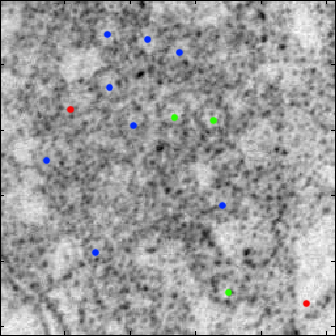
\includegraphics[scale=0.65]{files/postmethod/img/ves1+2_th-30_res2.png}
	\end{minipage}
	\hspace{0.5cm}
	\begin{minipage}[b]{0.5\linewidth}
		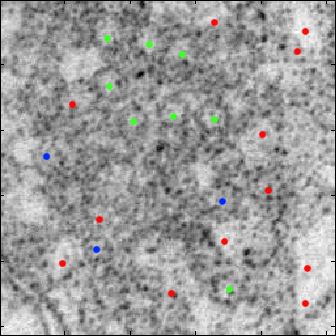
\includegraphics[scale=0.65]{files/postmethod/img/ves1+2_th-34_res2.png}
	\end{minipage}
	\caption{Til venstre ses resultatet efter foldning med vesikel A og C og tærskelværdi på 30\%. Til højre ses samme foldning bare med tærskelværdi på 34\%. Grønne er korrekt detekterede vesikler. Røde er forkert detekterede vesikler. Blå er vesikler der ikke blev detekteret.\label{fig:postmethod_conv_ves_1}}
\end{figure}

Dette virker som et ret fint resultat, da vi ved hjælp af 2 vesikler rent faktisk kan finde 8 i alt. For at undersøge hvorvidt dette resultat også er gældende for andre celler, vil vi undersøge resultatet ved at vælge en anden celle fra samme oprindelige billede, hvor indstillingerne på cameraet altså er ens som hvor vi har cellerne fra, og dernæst vælge en celle fra et helt andet billede. Målet med dette er altså at se hvor gode vores vesikler er til at finde andre vesikler i nye områder.

Først vælger vi et område der ligger en anelse længere nede end det område hvor vesikel A og C er taget fra. Formålet med dette er at se om de kan benyttes til at finde flere vesikler i samme billede. I figur \ref{fig:postmethod_conv_area3} ses området som vi har valgt, og i figur \ref{fig:postmethod_conv_gt3} har vi markeret ground truth i billedet.

\begin{figure}[H]
		\centering
		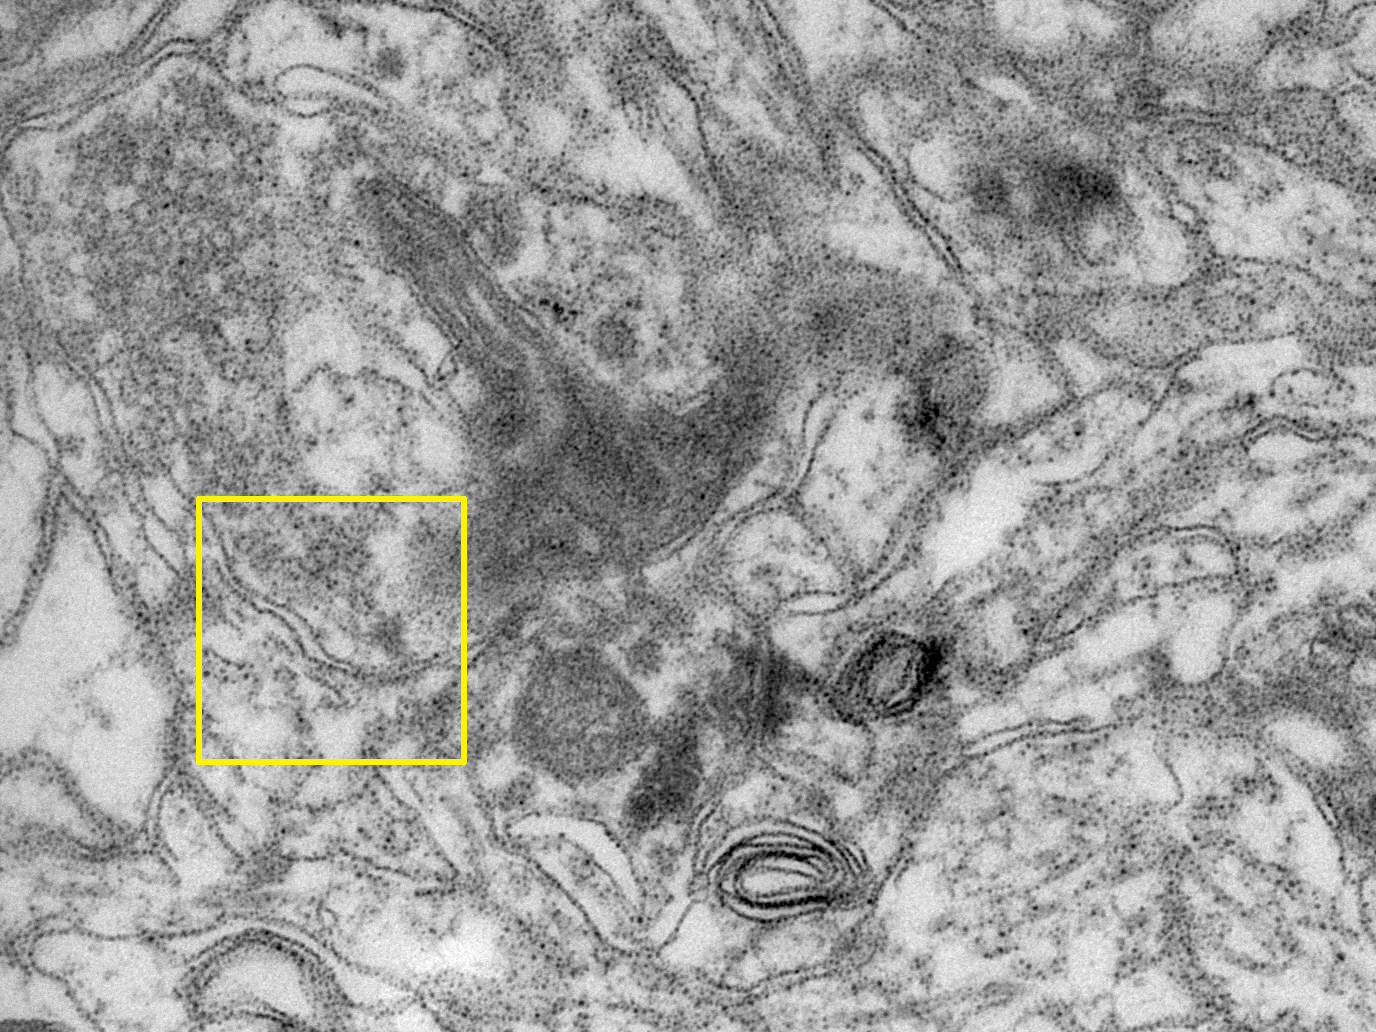
\includegraphics[scale=0.5]{files/postmethod/img/area_3.png}
	\caption{Området i det originale billede som vi er interesseret i.\label{fig:postmethod_conv_area3}}
\end{figure}

\begin{figure}[H]
		\centering
		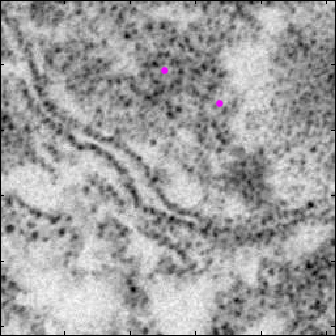
\includegraphics[scale=0.65]{files/postmethod/img/ground_truth3.png}
	\caption{Ground truth markeret med pinke prikker i et udsnit af en celle.\label{fig:postmethod_conv_gt3}}
\end{figure}

Da vi i de ovenstående forsøg fik de bedste resultater med en tærskelværdi på 34\%, vil vi også prøve at danne det nye billede med denne tærskelværdi. Resultatet ses i figur \ref{fig:postmethod_conv_post_img3_th34}, hvor det tydeligt fremgår at der findes alt for meget. Vi forsøger os i stedet med alle tærskelværdier fra 1\% til 34\%, og finder det bedste resultat ved 6\%. Dette ses i figur \ref{fig:postmethod_conv_post_img3_th6}. Her ser vi at vesikel A og C tilsammen har fundet begge de ønskede vesikler, og har så fundet 5 falske positive. Dette giver en sand-positiv-ratio på $1$ og en fejl ratio på $0.714$.

\begin{figure}[H]
		\centering		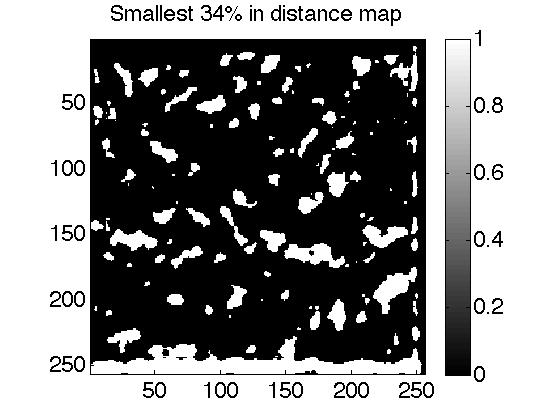
\includegraphics[scale=0.65]{files/postmethod/img/ves1+2_img3_th-34.png}
	\caption{Resulterende distance map efter en tærskelværdi på 34\%. De hvide områder er de steder algoritmen har fundet vesikler.\label{fig:postmethod_conv_post_img3_th34}}
\end{figure}

\begin{figure}[H]
		\centering
	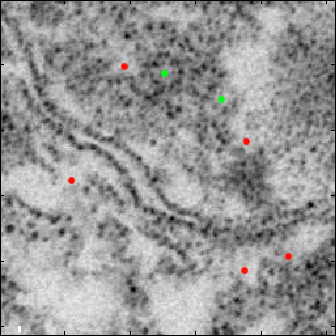
\includegraphics[scale=0.65]{files/postmethod/img/ves1+2_img3_th-6.png}
	\caption{Resultatet efter en tærskelværdi på 6\% hvor hvert område efterfølgende er markeret med en farve i det originale celleudsnit. Grønne er korrekt detekterede vesikler. Røde er forkert detekterede vesikler. Blå er vesikler der ikke blev detekteret.\label{fig:postmethod_conv_post_img3_th6}}
\end{figure}

Vi har til det næste udsnit valgt et helt andet billede. Som det fremgår virker billedet lysere end det første, hvorfor det bliver interessant at se påvirkningen ved at folde med vores vesikler i dette område. I figur \ref{fig:postmethod_conv_area2} har vi markeret hvor på billedet udsnittet er taget, og i figur \ref{fig:postmethod_conv_gt2} har vi markeret ground truth i cellen. Her skal vi altså finde 6 vesikler.

\begin{figure}[H]
		\centering
		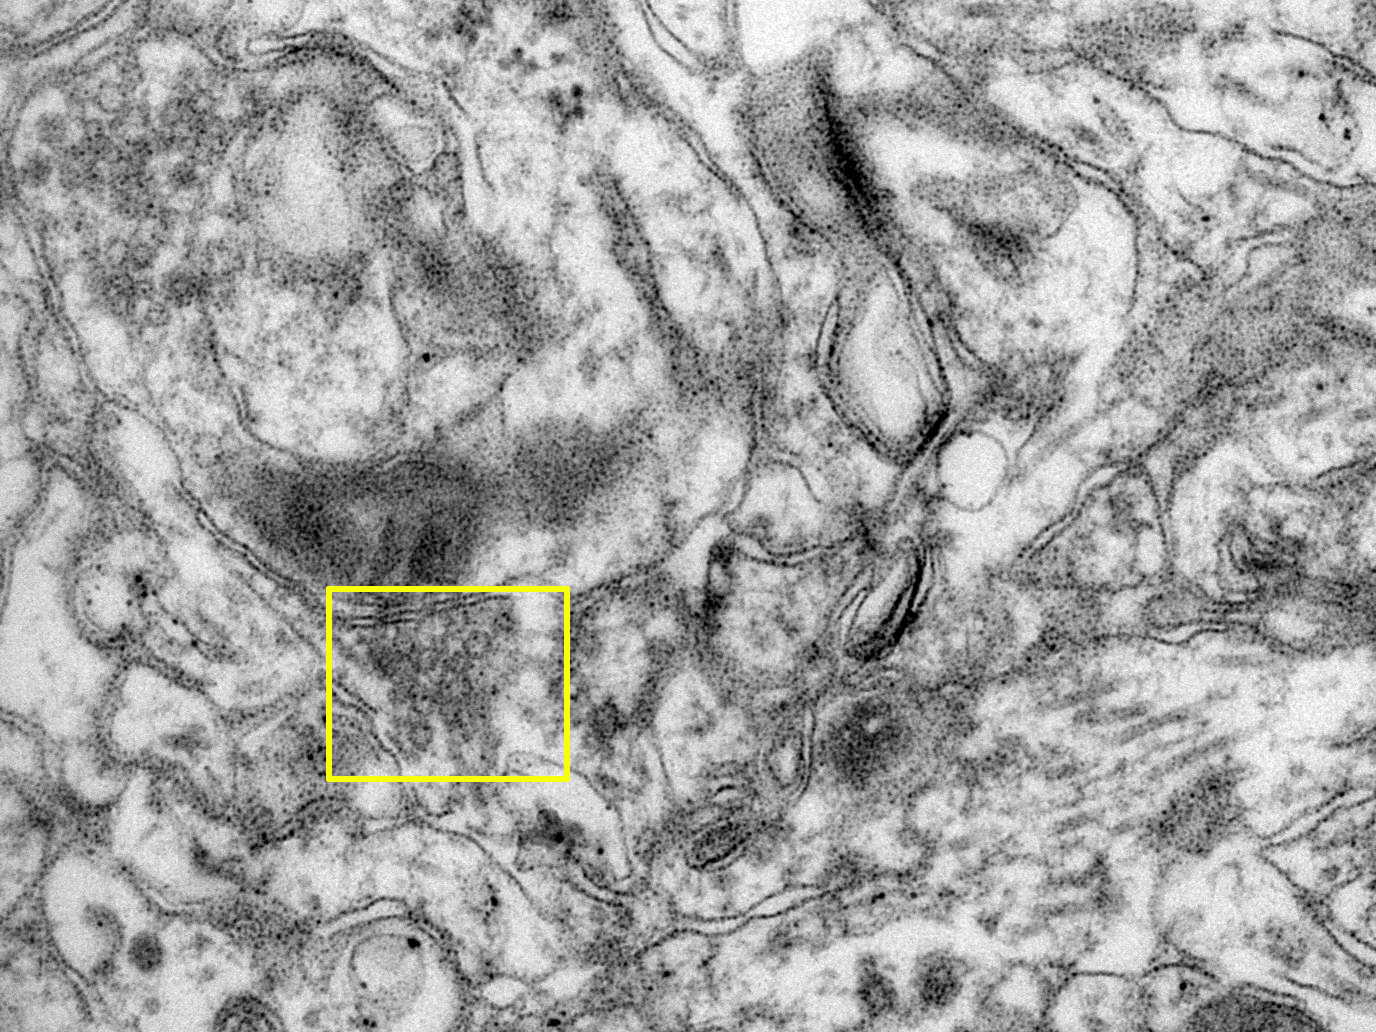
\includegraphics[scale=0.5]{files/postmethod/img/area_2.png}
	\caption{Området i det originale billede som vi er interesseret i.\label{fig:postmethod_conv_area2}}
\end{figure}

\begin{figure}[H]
		\centering
		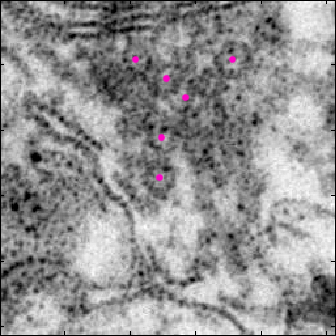
\includegraphics[scale=0.65]{files/postmethod/img/ground_truth2.png}
	\caption{Ground truth markeret med pinke prikker i et udsnit af en celle.\label{fig:postmethod_conv_gt2}}
\end{figure}

Nedenstående billede i figur \ref{fig:postmethod_conv_post_img2_th34} er resultatet efter en tærskelværdi på 34\%. Dette er tydeligvis ikke godt, og vi forsøger os i stedet med langt lavere tærskelværdier. De bedste resultater fås ved en tærskelværdi på 5\%. Det resulterende billede hvor resultaterne er påtegnet ses i figur \ref{fig:postmethod_conv_post_img2_th5}. Her ser vi at der er detekteret 2 korrekte vesikler, 6 vesikler er detekteret forkert og der mangler at detekteres 4 vesikler. Dette giver en sand-positiv-ratio på $0.333$ og en fejl-ratio på $0.75$. Til at danne dette billede har vi igen kombineret resultaterne fra vesikel A og vesikel C's foldning med billedet. Vesikel C står dog kun for en enkelt falsk positiv, hvor resten af de detekterede områder er fra foldningen med vesikel A.

\begin{figure}[H]
		\centering		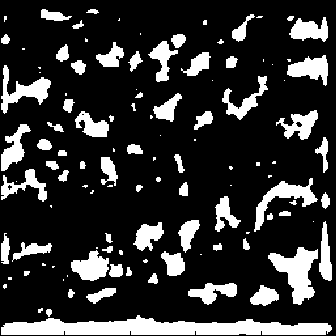
\includegraphics[scale=0.65]{files/postmethod/img/ves1+2_img2_th-34.png}
	\caption{Distance map efter tærskelværdi på 34\%.\label{fig:postmethod_conv_post_img2_th34}}
\end{figure}

\begin{figure}[H]
		\centering
	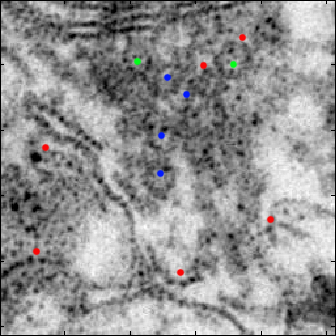
\includegraphics[scale=0.65]{files/postmethod/img/ves1+2_img2_th-5.png}
	\caption{Resultatet efter en tærskelværdi på 5\% hvor hvert område efterfølgende er markeret med en farve i det originale celleudsnit. Grønne er korrekt detekterede vesikler. Røde er forkert detekterede vesikler. Blå er vesikler der ikke blev detekteret.\label{fig:postmethod_conv_post_img2_th5}}
\end{figure}

Fra disse undersøgelser kan vi altså konkludere at vesikel A og C finder 72.7\% af vesiklerne i billedet hvor de er taget fra, 100\% af et andet område fra samme billede, og 33\% af vesiklerne i et nyt billede. Dette er selvfølgelig ikke automatisk gældende for alle områder vi ser på, men allerede nu kan vi se en tendens til at vesiklerne bedst finder andre vesikler i områder der ligner det område hvor de er taget fra.

Vi vil derfor afsøge muligheden for en udvidelse af vores algoritme der gør at vi kan vægte vores fundne områder. Hvis vi i et billede har fundet 9 mulige vesikler efter foldning med en eksempelvesikel, og en ny algoritme så fortæller os at den har fundet 6 mulige vesikler, vil vi kunne sammenholde disse resultater, og de steder de begge finder vesikler vil der være større sandsynlighed for at der rent faktisk er en vesikel.

\subsection{Sparse Label Dictionaries}	% Marcus
%\textbf{Disclaimer der måske skal med: SLD er en metode udviklet af Anders noget fra DTU, vi har set metoden til et foredrag men har ikke set noget litteratur der beskriver metoden udførligt. Dette er derfor vores udlægning af SLD-metoden}\\

Sparse Label Dictionaries metoden (SLD) har til formål at segmentere billeder. SLD opretholder to matricer med information om image patches, den ene indeholder intensiteten og den anden den assosierede label information.

SLD opbygger disse to matricer i to trin, første trin er at initialisere matricen. Dette gøres ved at se på to billeder, et træningsbillede samt et billede hvor ground truth er markeret. Fra starten vælges så en størrelse på det udsnit man ønsker at arbejde med. Et atom klippes så ud af træningsbilledet i pixel (0,0) og med størrelse $\sqrt{n}\times\sqrt{n}\times h$, hvor $n$ er antallet af pixels i udsnittet og h er farvedybten, så f.eks. 1 ved grayscale og 3 ved RGB billeder. Denne atom gemmes så i intensitetsmatricen. I præcis samme område klippes en atom ud af ground truth billedet der så gemmes i labelmatricen. En skematisk illustration af denne proces ses i figur \ref{fig:postmethod_intensitydict_init}. Ground truth billedet har også h dimensioner, hvor hvert segment der ønskes at detekteres er markeret men en farve. Vores udsnit flyttes så en pixel, hvorefter det samme gøres igen. Det vil sige at hvis træningsbilledet er $m\times m$ og vores atom størrelse er $n\times n$ så samler vi $(m-n+1)^2$ billeder. 

\begin{figure}[H]
		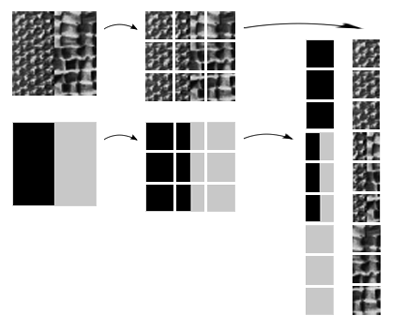
\includegraphics[scale=1]{files/postmethod/img/dict_new1.png}
	\caption{Figuren illustrerer hvordan træningsbilledet hhv. ground truth billedet bliver opdelt i atomer og placeret i intensitetsmatricen hhv. labelmatricen repræsenteret ved søjlerne til højre i figuren. \label{fig:postmethod_intensitydict_init}}
\end{figure}

For at bygge de mest optimale billeder, ønsker vi at labelmatricen indeholder unikke billeder for hver klasse. Dette gøres ved at der vælges et tilfældigt subset af udsnittene fra træningsbilledet, og ved en iterativ proces, undersøges det hvorvidt det associerede labelatom allerede er tilnærmelsesvis repræsenteret i labelmatricen, og tilføjes kun hvis det ikke er tilfældet. Dette sikrer både at størrelsen på matricerne bliver minimeret der gør at listen er hurtigere at gennemgå, samt at billedudsnit med lignende intensiteter og labels tilhører samme matriceatomer. 

Når matricerne er fyldt op med intensitet- og labelatomer begynder en ny algoritme at optimere på matricernes indhold. Ideelt set vil en pixel i et labelatom have sandsynligheden 1 for en klasse og 0 for alle andre klasser. Algoritmen forsøger at opnå dette ved iterativt at opdele atomerne i klasser og redigere i label sandsynlighederne. 

Med de færdigbyggede matricer kan SLD gå igang med at segmentere billeder. Metoden starter typisk med at modtage et testbillede der bare kan være testbilledet med akserne ombyttet. Denne proces er dog kun for at teste at de matricer man har opbygget rent faktisk kan segmentere de klasser man ønsker.

Processen med at segmentere et billede med de to matricer starter ligesom når matricerne blev opbygget. Udsnit størrelsen på $\sqrt{n}\times\sqrt{n}$ vælges, hvor $n$ igen er antallet af pixels i udsnittet, og løber igennem det billede der ønskes segmenteret på samme vis som da vi fyldte matricerne. For hvert udsnit findes det atom, $d^*$, i intensitetsmatricen som euklidisk ligger tættest på billedudsnittet ved ligningen
\begin{align}
	d^* = min_j ||d_j-x||
\end{align}

Herefter hentes den tilsvarende label ud fra labelmatricen og tilføjes til det nye segmenterede billede. Hver atom man tilføjer til det nye billede adderes oveni de allerede indsatte pixels hvilket betyder at hver pixel i det resulterende billede består af bidrag fra $n$ labelatom pixels, og som er et gennemsnit af sandsynlighederne af alle labels der dækker denne pixel. Denne labeling proces ses illustreret i figur \ref{fig:postmethod_sld_labelpatch}.  

Når SLD algoritmen er færdig vil det resulterende billede være segmenteret, et eksempel ses i figur \ref{fig:postmethod_sld_resulting}.

\begin{figure}[H]
		\centering
		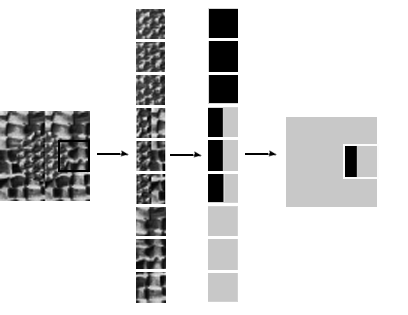
\includegraphics[scale=0.8]{files/postmethod/img/dict_new2.png}
	\caption{\label{fig:postmethod_sld_labelpatch}}
\end{figure}

\begin{figure}[H]
		\centering
		
\includegraphics[scale=1]{files/postmethod/img/dict_new3.png}
	\caption{\label{fig:postmethod_sld_resulting}}
\end{figure}

Skaberne af SLD beskriver metoden som værende en forbedring i forhold til andre lignende metoder, da den kun indeholder én matrice af intensitetsatomer selvom der er flere klasser. Samtidig er metoden stærk selv overfor billeder med meget støj og træningsbilleder med labels i dårlig kvalitet. I figur \ref{fig:postmethod_sld_testing} vises i første linje tre testbilleder med hhv. 5, 16, 10 og 2 klasser der skal segmenteres. I anden linje ses ground truth af disse billeder. I tredie linje ses resultatet efter segmenteringen. Her ses det tydeligt at hver klasse er segmenteret og der kun er segmenteringsfejl i overgangen mellem klasserne. Billederne er bl.a. behandlet med et gaussisk filter med standard afvigelse på 1.5 og udsnitstørrelse på $3\times3$.

\begin{figure}[H]
		\centering
		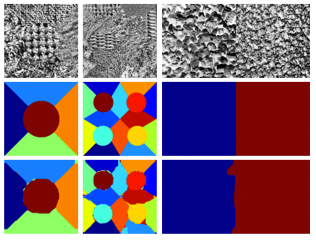
\includegraphics[scale=1]{files/postmethod/img/dict_6.png}
	\caption{Testbilleder øverst, ground truth i midten og resultatet af segmenteringen nederst.\label{fig:postmethod_sld_testing}}
\end{figure}

\subsection{Vores implementation af SLD}
Der er flere ting som SLD understøtter, som vi ikke har brug for til at løse opgaven for os. En af disse ting er at SLD er designet til at klassificere lige så mange klasser som man har brug for, hvor vi kun skal segmentere 2 klasser. Da vi ikke har så mange klasser, har vi naturligvis ikke så mange atomer i vores matricer, og behovet for at optimere ved at fjerne atomer så der kun er unikke atomer er selvfølgelig ikke lige så stort. I vores implementation af SLD har vi altså valgt at holde det helt simpelt. Vi opbygger ligeledes to matricer bestående af atomer fra et træningsbillede og de tilhørende labelatomer fra et ground truth billede. Når vi så vil segmentere et billede løber vi listen af atomer igennem og finder atomet med kortest euklidisk afstand og adderer den tilsvarende label i det resulterende billede. I figur \ref{fig:postmethod_sld_train1} ser vi et træningsbillede der er et udsnit fra billedet længst til højre i figur \ref{fig:postmethod_sld_testing}, samt det tilhørende ground truth billede. Ground truth billedet har fået efterfølgende markeret en sort kant omkring det for at vise afgrænsningen af den hvide side. I figur \ref{fig:postmethod_sld_label1} ser vi så billedet hvor SLD har fundet træningsbilledet igen. Som vi kan se finder algoritmen området som ønsket. Bemærk igen at kanten ikke er fundet korrekt, da algoritmen ikke er designet til at klare kanten. % Uddyb? 
Vi har benyttet en atomstørrelse på 7 pixels. % Omskriv / Flyt

\begin{figure}[H]
	\begin{minipage}[b]{0.5\linewidth}
		\centering
		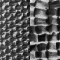
\includegraphics[scale=3]{files/postmethod/img/imTrain.png}
	\end{minipage}
	\hspace{0.5cm}
	\begin{minipage}[b]{0.5\linewidth}
		\centering
		
\includegraphics[scale=3]{files/postmethod/img/imGT.png}
	\end{minipage}
	\caption{...\label{fig:postmethod_sld_train1}}
\end{figure}

\begin{figure}[H]
		\centering
		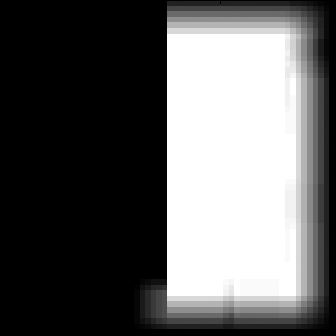
\includegraphics[scale=0.54]{files/postmethod/img/sld_preres1.png}
	\caption{...\label{fig:postmethod_sld_label1}}
\end{figure}

Vi har så lavet et testbillede for at undersøge hvorvidt algoritmen kan finde samme mønstre, bare i en ny figur. Vi har her taget mønsteret til højre i træningsbilledet og duplikeret så det fylder hele billedet. Herefter har vi taget mønsteret til venstre og lagt som en cirkel i centrum af billedet. Resultatet ses til venstre i figur \ref{fig:postmethod_sld_res1}. Til højre i samme billede ses vores SLD algoritmes forsøg på at segmentere figuren. Resultatet er vi tilfredse med, da mønsteret til venstre i træningsbilledet, som vi fra starten af har sagt skal repræsenteres som sort i labelmatricen, fremgår tydeligt i midten af det nye billede.

% Kommenter at vi går ud fra pixlen og atomXatom opXned i stedet for som centerpixel??

\begin{figure}[H]
	\begin{minipage}[b]{0.5\linewidth}
		\centering
		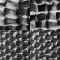
\includegraphics[scale=3]{files/postmethod/img/imTest.png}
	\end{minipage}
	\hspace{0.8cm}
	\begin{minipage}[b]{0.5\linewidth}
		\centering
		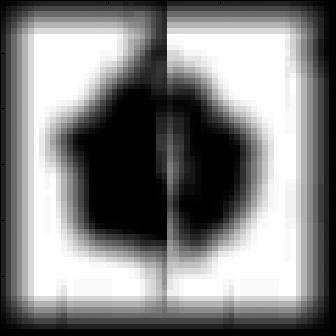
\includegraphics[scale=0.54]{files/postmethod/img/sld_res1.png}
	\end{minipage}
	\caption{...\label{fig:postmethod_sld_res1}}
\end{figure}

Tilfredse med vores algoritme ser vi nu i stedet på vores cellebilleder. Vi starter igen med at konstruere et træningsbillede samt et ground truth billede ud fra dette træningsbillede. For at formindske udregningstiden har vi valgt et udsnit af dette billede, et $100\times100$ pixel udsnit fra \ref{fig:postmethod_conv_gt} af de 4 vesikler der er samlet på en række. Resultatet af dette ses i figur \ref{fig:postmethod_sld_train2}.

\begin{figure}[H]
	\begin{minipage}[b]{0.5\linewidth}
		\centering
		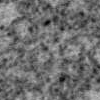
\includegraphics[scale=3]{files/postmethod/img/imTrain2.png}
	\end{minipage}
	\hspace{0.5cm}
	\begin{minipage}[b]{0.5\linewidth}
		\centering
		
\includegraphics[scale=3]{files/postmethod/img/imGT2.png}
	\end{minipage}
	\caption{...\label{fig:postmethod_sld_train2}}
\end{figure}

Vi har herefter set på størrelsen af vores atomer. Forfatterne af SLD har bedst erfaringer med $3\times3$ atomer til at fange detaljerne i deres billeder. I vores billede derimod har vi brug for større plads til at vise et stykke vesikel på. I figur \ref{fig:postmethod_ves_grid} har vi markeret et gitter der svarer til $7\times7$ pixel atomstørrelser. Som det fremgår er denne størrelse nødvendig for at få begge sider af en kant med, hvilket er hvad adskiller en vesikel fra almindelig støj, som vi tidligere har været inde på. %ref evt. til afsnittet om pixelfarveværdier?
At vores algoritme kan segmentere træningsbilledet igen fremgår tydeligt af figur \ref{fig:postmethod_sld_label2}.

\begin{figure}[H]
		\centering
		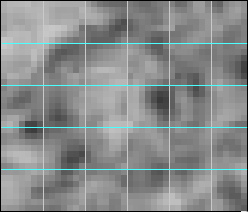
\includegraphics[scale=1]{files/postmethod/img/ves_grid.png}
	\caption{...\label{fig:postmethod_ves_grid}}
\end{figure}

\begin{figure}[H]
		\centering
		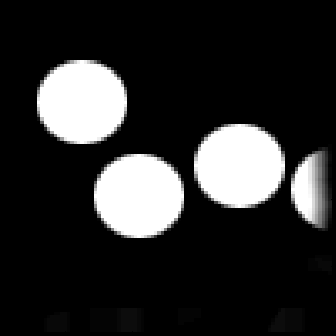
\includegraphics[scale=0.54]{files/postmethod/img/sld_preres2.png}
	\caption{...\label{fig:postmethod_sld_label2}}
\end{figure}

I vores test af algoritmen lavede vi nu et nyt billede ved at flytte rundt på mønstrene i træningsbilledet. Dette er dog ikke muligt i cellebilledet. I stedet vælger vi et testbillede der kommer fra samme celle, bare længere oppe. Billedet, vist i figur \ref{fig:postmethod_sld_res2}, indeholder 4 vesikler vi ønsker at segmentere. Nederst ses en vesikel markeret med blåt, det er den øverste vesikel i træningsbilledet, og vi forventer naturligvis at denne kan segmenteres korrekt igen. De tre andre vesikler er nye vesikler som algoritmen skal segmentere.

\begin{figure}[H]
	\begin{minipage}[b]{0.5\linewidth}
		\centering
		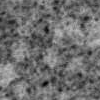
\includegraphics[scale=3]{files/postmethod/img/imTest2.png}
	\end{minipage}
	\hspace{0.8cm}
	\begin{minipage}[b]{0.5\linewidth}
		\centering
		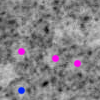
\includegraphics[scale=3]{files/postmethod/img/sld_gt3.png}
	\end{minipage}
	\caption{...\label{fig:postmethod_sld_res2}}
\end{figure}

\begin{figure}[H]
	\begin{minipage}[b]{0.5\linewidth}
		\centering
		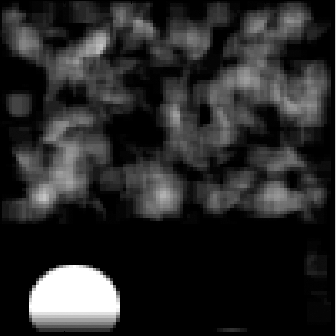
\includegraphics[scale=0.54]{files/postmethod/img/sld_res2.png}
	\end{minipage}
	\hspace{0.8cm}
	\begin{minipage}[b]{0.5\linewidth}
		\centering
		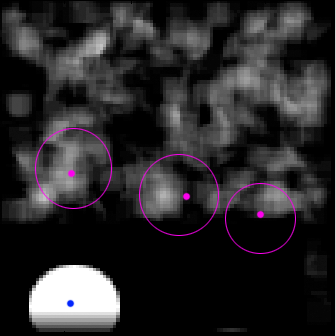
\includegraphics[scale=0.54]{files/postmethod/img/sld_res22.png}
	\end{minipage}
	\caption{...\label{fig:postmethod_sld_res22}}
\end{figure}

I figur \ref{fig:postmethod_sld_res22} ser vi resultatet. Til venstre i figuren ses det nye billede bygget med vores SLD algoritme, og til højre er de områder vi ønskede at segmentere markeret med cirkler. Som det tydeligt ses er der intet der adskiller disse områder fra resten af billedet. Vi kan derfor ikke bruge resultatet her til at segmentere områder. Vi prøver derfor at ændre på vores billeder.

Første ændring er at vi ændrer i ground truth i forhold til træningsbilledet. Som vi tidligere har været inde på er kanten en stor del af det der definerer en vesikel fordi mønsteret i centrum kan minde om den almindelige baggrund i en celle. Vi har derfor klippet hvad der svarer til dette centrum ud af ground truth, i håb om at billedet så bliver mere korrekt. I figur \ref{fig:postmethod_sld_gt4} nedenfor ses til venstre det nye ground truth billede, og til højre det resulterende billede fra segmenteringen af vores testbillede. Igen er resultatet ikke godt da vi heller ikke her kan se tydelige mønstre hvor vesiklerne burde være.

\begin{figure}[H]
	\begin{minipage}[b]{0.5\linewidth}
		\centering
		
\includegraphics[scale=3]{files/postmethod/img/imGT3.png}
	\end{minipage}
	\hspace{0.8cm}
	\begin{minipage}[b]{0.5\linewidth}
		\centering
		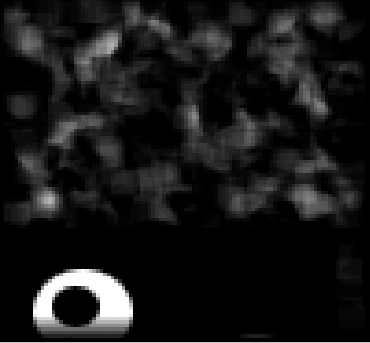
\includegraphics[scale=0.42]{files/postmethod/img/sld_res3.png}
	\end{minipage}
	\caption{...\label{fig:postmethod_sld_gt4}}
\end{figure}

Næste ændring er så at udglatte billedet. Dette har vi tidligere forsøgt, men det gav intet godt resultat i forhold til de funktioner vi prøvede der. % Henvis til afsnittet!
Da vi med denne algoritme prøver at finde kanterne, kan det dog være smart at udglatte igen. Til dette har vi brugt et gaussfilter med en kerne på $\sigma=2$. %Tjek! Det er fra photoshop!
Vi har både udglattet træningsbilledet samt testbilledet, disse ses i figur \ref{fig:postmethod_sld_res3}, og har efterfølgende bygget vores matricer op med atomstørrelser på $7\times7$ pixels.

\begin{figure}[H]
	\begin{minipage}[b]{0.5\linewidth}
		\centering
		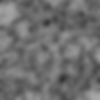
\includegraphics[scale=3]{files/postmethod/img/imTrain3.png}
	\end{minipage}
	\hspace{0.8cm}
	\begin{minipage}[b]{0.5\linewidth}
		\centering
		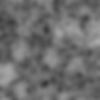
\includegraphics[scale=3]{files/postmethod/img/imTest5.png}
	\end{minipage}
	\caption{...\label{fig:postmethod_sld_res3}}
\end{figure}

Som det fremgår af billedet til venstre i figur \ref{fig:postmethod_sld_res5} finder vi nu især tre områder foruden den kendte vesikel der fremtræder. I billedet har vi med ringe markeret de steder vi ved der er vesikler. Vi har i billedet til højre i samme figur konstrueret billedet efter en tærskelværdi. Som det ses finder algoritmen fire områder. To af områderne ligger korrekt inden for en vesikel, området i bunden er den allerede kendte vesikel og området i toppen er et fejldetekteret område. 

\begin{figure}[H]
	\begin{minipage}[b]{0.5\linewidth}
		\centering
		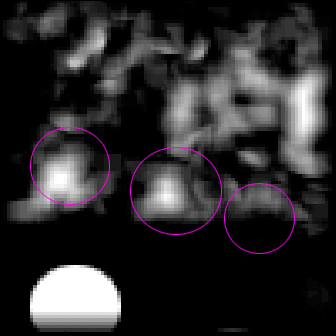
\includegraphics[scale=0.54]{files/postmethod/img/sld_res5.png}
	\end{minipage}
	\hspace{0.8cm}
	\begin{minipage}[b]{0.5\linewidth}
		\centering
		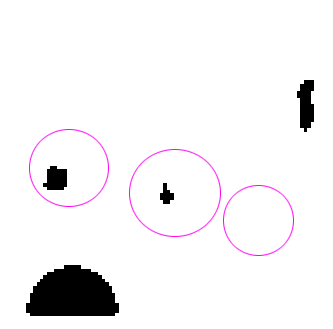
\includegraphics[scale=0.54]{files/postmethod/img/sld_res6.png}
	\end{minipage}
	\caption{...\label{fig:postmethod_sld_res5}}
\end{figure}

Dette resultat er rigtig positivt , men for at vi kan sige noget mere om metoden skal den også kunne finde områder der ikke er kendt, altså vesikler i ukendte celler. Vi har derfor igen taget fat i områderne fra \ref{fig:postmethod_conv_gt3} og \ref{fig:postmethod_conv_gt2}, og har udglattet begge disse områder med et gaussfilter ligesom med billedet ovenfor. Billederne i figur \ref{fig:postmethod_sld_res6} er det resulterende billede samt det samme billede efter en tærskelværdi. I begge billeder har vi med ringe markeret hvor vi ved der skulle findes vesikler. Som det tydeligt fremgår af billederne er vesiklerne ikke korrekt segmenteret.

Vi forsøger os da med det næste område, som altså er det udglattede billede af figur \ref{fig:postmethod_conv_gt2}. Igen viser vi i figur \ref{fig:postmethod_sld_res7} det resulterende billede samt billedet efter en tærskelværdi, hvor vi har indsat ringe for at markeret ground truth. Vi kan se at der er segmenteret områder, men kun et af områderne ligger indenfor cirklerne.

\begin{figure}[H]
	\begin{minipage}[b]{0.5\linewidth}
		\centering
		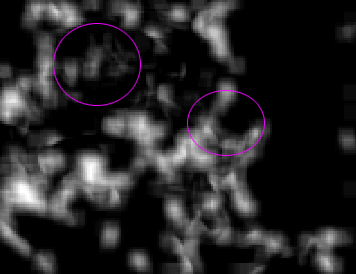
\includegraphics[scale=0.54]{files/postmethod/img/sld_res8.png}
	\end{minipage}
	\hspace{0.8cm}
	\begin{minipage}[b]{0.5\linewidth}
		\centering
		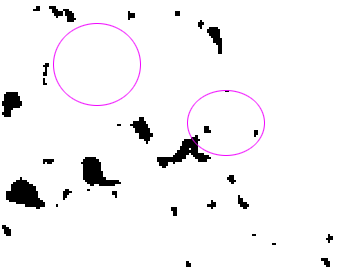
\includegraphics[scale=0.54]{files/postmethod/img/sld_res9.png}
	\end{minipage}
	\caption{...\label{fig:postmethod_sld_res6}}
\end{figure}

\begin{figure}[H]
	\begin{minipage}[b]{0.5\linewidth}
		\centering
		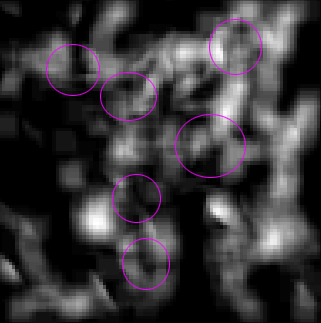
\includegraphics[scale=0.54]{files/postmethod/img/sld_res10.png}
	\end{minipage}
	\hspace{0.8cm}
	\begin{minipage}[b]{0.5\linewidth}
		\centering
		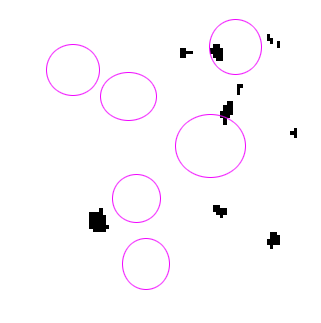
\includegraphics[scale=0.54]{files/postmethod/img/sld_res11.png}
	\end{minipage}
	\caption{...\label{fig:postmethod_sld_res7}}
\end{figure}

Vi må altså konstatere at vores SLD algoritme er ganske god til at segmentere vesikler fra samme celle som matricerne med atomer er bygget af, men så snart vi bevæger os udenfor cellen til andre celler og vesikler, har algoritmen problemer. Det faktum at vi rent faktisk fandt 2 ud af 3 ukendte vesikler i samme celle som matricen var bygget efter, fortæller os samtidig af metoden virker, det kræver dog at vi bygger matricerne med repræsentative atomer for mønstrene. Det sidste er dog en stor udfordring da vesiklerne ikke har en generel struktur og matricerne skal derfor bestå af atomer fra mange forskellige vesikler. I vores matricer har vi haft ca. 9000 atomer i hver matrice, hvor et udsnit på $100\times100$ pixel tager ca. 20 minutter at segmentere for vores implementation af SLD i \texttt{Matlab}. I SLD har forfatterne forsøgt sig med forskellige matricestørrelser. Deres matricer indeholder f.eks. 50.000 atomer, men pga. deres optimeringsalgoritmer før segmenteringen kan de vælge de atomer der passer bedst til at segmentere et ønsket mønster og dermed bringe antallet af atomer i matricerne ned til ca. 30.000. Denne reduktion af matricerne er en mulig optimering der ville gøre udførselstiden hurtigere. 

En anden mulig optimering for vores implementation af SLD algoritmen er at indføre en tærskelværdi for hvor langt afstanden må være fra et udsnit og dets valgte atom, da man så kun ville tilføje labels til det resulterende billede, hvis det tilsvarende intensitetsatom lignede udsnittet godt, og ikke bare blev valgt fordi det lignede bedst af dem der nu var. Som det er nu, skabes der en ikke-linearitet, hvis f.eks. udsnit A har euklidisk afstand x fra intensitetsatom C, og udsnit B har euklidisk afstand y fra intensitetsatom C, hvor x $>$ y, så får de alligevel begge tildelt intensitetsatom C's tilsvarende label. Her kunne man vægte graden af betydning denne label får i det endelige billede efter hvor godt afstanden passede, og dermed skabe en større linearitet. 

Vi har dog valgt ikke at arbejde videre med SLD algoritmen da denne kun var til for at skabe mere tillid til resultaterne der findes ved at folde med en vesikel. \\

\subsection{Evaluering}
I tidligere afsnit har vi beskrevet metoden \emph{Segmentering med eksempelbilleder}. Vi fik her segmenteret en ukendt vesikel med en sand-positiv-ratio på 33\%. Vi ønskede at forbedre dette resultat ved at benytte flere segmenteringsalgoritmer, og introducerede da SLD. Da vi ikke kunne få et godt resultat med ukendte billeder, selv med forskellig behandling af billederne algoritmen benyttede sig af, valgte vi ikke at gå videre med kombinationen af de to metoder. Vores endelige program består da udelukkende af metoden udviklet i \emph{Segmentering med eksempelbilleder} afsnittet, og det er den vi nu vil evaluere resultaterne af.

Metoden går i al simpelhed ud på at segmentere en celle ved i hver pixel at udregne den euklidiske afstand til en vesikel, og gemme resultaterne i et nyt distance map. Ved at køre en tærskelværdi på resultatet får vi de segmenterede områder frem. Ved at kombinere resultaterne efter flere segmenteringer med forskellige vesikler, kunne vi opnå et bedre resultat. 

Som nævnt i forordsafsnittet har vi sent i projektet modtaget nye cellebilleder. Vi vil nu afprøve vores segmenteringsprogram på disse nye billeder. Vi har udvalgt to celler fra disse billeder som vi ønsker at segmentere. Vi har for hver af områderne valgt 3 vesikler, så vi i alt kan finde afstand med 6 forskellige vesikler. I figur \ref{fig:animalsss} (a)-(f) ses første celle hvor hver af de 6 billeder svarer til segmentering med en enkelt vesikel. Ved at observere på resultaterne finder vi at de bedste billeder blev fundet ved en tærskelværdi på omkring 34\% ligesom vi har konkluderet tidligere i tabel \ref{tab:postmethod_tabelll}, og vi har i de resulterende billeder markeret SP, FP og FN. I figur \ref{fig:animalssssssssssss} ses segmenteringen med de samme 6 vesikler, bare på en ny celle.

Vi er altså interesserede i at vide hvor mange af vesiklerne vores program finder, og hvor ofte det detekterer områderne forkert. Denne trade-off fanges mest præcist ved en recall-precision kurve.

Den første ting vi er interesserede i, antallet af detekterede vesikler, bliver angivet ved recall. 
\begin{align}
	Recall &= \frac{\textit{Antal korrekte positive}}{\textit{Total antal positive i datasættet}}
\end{align}
Den anden ting vi er interesserede i, antallet af falske detektioner relativ til det totale antal detektioner, er angivet ved \emph{1-precision}.
\begin{align}
	1-Precision &= \frac{\textit{Antal falske positive}}{\textit{Antal korrekte positive + Antal falske positive}}
\end{align}
Ved at plotte \emph{recall} imod \emph{(1-precision)} udtrykkes det ønskede tradeoff. Dette har vi gjort i figur \ref{fig:postmethod_recallprec} hvor de røde cirkler er fra resultaterne fra de nye billeder og de 3 blå cirkler er de tidligere resultater med vesikel A, B og C med tærskelværdi på 34\% fra tabel \ref{tab:postmethod_tabelll}. De røde cirkler er resultaterne fra figur \ref{fig:animalsss} (a)-(f) og \ref{fig:animalssssssssssss} (a)-(f). 

Her kan vi aflæse at vi har fået en klar forbedring af fejlraten i forhold til resultaterne fundet med de tidligere billeder da de røde cirkler er placeret fra ca. 0.2 til 0.5 på x-aksen imod de gamle resultater der er placeret fra ca. 0.4 til 0.8. Recall-værdien, som er sand-positiv-ratioen fra tidligere, kan vi også aflæse en klar forbedring af. En anden bemærkelsesværdig observation er at de røde cirkler er relativt pænt samlet. I de tidligere afsnit observerede vi at cellebilleder hvor man fandt afstand til vesikler fra samme celle blev klart bedre segmenteret end hvis vesiklerne var fra en anden celle. Denne observation gør sig ikke gældende med de nye billeder. Da resultaterne er så mærkbart bedre med de nye billeder, vil vi i den resterende del af evalueringen kun benytte disse.

\begin{figure}[H]
	\centering
	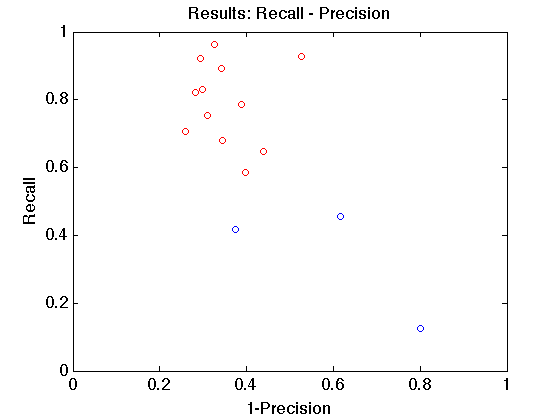
\includegraphics[scale=0.9]{files/postmethod/img/recallvsprecision.png}
	\caption{Recall vs. 1-precision plottet fra resultaterne vist i figur \ref{fig:animalsss} og \ref{fig:animalssssssssssss}.\label{fig:postmethod_recallprec}}
\end{figure}

Som beskrevet kan vi nu kombinere de segmenterede billeder og se på de resultaterne dette medfører. Spørgsmålet er bare hvor mange af billederne vi skal kombinere. Vi har derfor i tabel \ref{tab:postmethod_tabel2222} forsøgt at kombinere ved først at vælge 2, 3, 4, 5 og til sidst 6 af resultaterne. Vi har derefter plottet \emph{Recall} vs. \emph{1-Precision} igen for disse nye resultater. Vi kan her aflæse at der sker en lille forbedring ved at kombinere to af resultaterne (blå cirkler) hvor den laveste \emph{recall} værdi er på $0.785$. Allerede ved at kombinere tre af resultaterne (grønne cirkler) får vi detekteret næsten alle vesiklerne uden at vores \emph{precision} forværres i for stor en grad. Vi ser samtidig at resultaterne ved at kombinere hhv. 4 (cyan cirkler), 5 (magenta cirkler) og 6 (sorte cirkler) forbedrer \emph{recall} værdien i en særlig grad, hvorimod \emph{precision} værdien forværres betydeligt her. Her kan vi altså konkludere at de bedste resultater blev opnået ved kombination af 3 tidligere resultater. 

\begin{table}
	\begin{tabular}{l|l|l|l|l|l|l}
		$\#$ & Billeder & SP & FP & FN & Recall & 1-Precision \\\hline
		2	&	\ref{fig:animalsss} (a)+(b)	&51	&26	&14 							&0.785 	&0.338\\\hline
		2	&	\ref{fig:animalsss} (c)+(d)	&51	&36	&14 							&0.785 	&0.414\\\hline
		2	&	\ref{fig:animalsss} (e)+(f)	&61	&42	&4 								&0.938 	&0.408\\\hline
		2	&	\ref{fig:animalssssssssssss} (a)+(b) &28 &31 &0 					&1 		&0.525\\\hline
		2	&	\ref{fig:animalssssssssssss} (c)+(d) &23	&14	&5 					&0.821 	&0.378\\\hline
		2	&	\ref{fig:animalssssssssssss} (e)+(f) &28	&20	&0 					&1 		&0.417\\\hline
		3	&	\ref{fig:animalsss} (a)+(b)+(c)	&60	&40	&5 							&0.923 	&0.4\\\hline
		3	&	\ref{fig:animalsss} (d)+(e)+(f)	&61	&61	&4 							&0.938 	&0.5\\\hline
		3	&	\ref{fig:animalssssssssssss} (a)+(b)+(c)	&28	&37	&0 				&1 		&0.578\\\hline
		3	&	\ref{fig:animalssssssssssss} (d)+(e)+(f)	&28	&26	&0 				&1 		&0.481\\\hline
		4	&	\ref{fig:animalsss} (a)+(b)+(c)+(d)	& 62 &52	&3 					&0.954 	&0.456\\\hline
		4	&	\ref{fig:animalssssssssssss} (a)+(b)+(c)+(d) &28	&39	&0 			&1 		&0.582\\\hline
		5	&	\ref{fig:animalsss} (a)+(b)+(c)+(d)+(e)	&62	&53	&3 					&0.954 	&0.461\\\hline
		5	&	\ref{fig:animalssssssssssss} (a)+(b)+(c)+(d)+(e)	&28	&41	&0 		&1 		&0.594\\\hline
		6	&	\ref{fig:animalsss} (a)+(b)+(c)+(d)+(e)+(f)	&63	&55	&2 				&0.969 	&0.466\\\hline
		6	&	\ref{fig:animalssssssssssss} (a)+(b)+(c)+(d)+(e)+(f) &28	&43 &0 	&1 		&0.606
	\end{tabular}
	\caption{Oversigt over resultaterne ved at kombinere flere billeder til et endeligt resultat.\label{tab:postmethod_tabel2222}}
\end{table}

\begin{figure}[H]
	\centering
	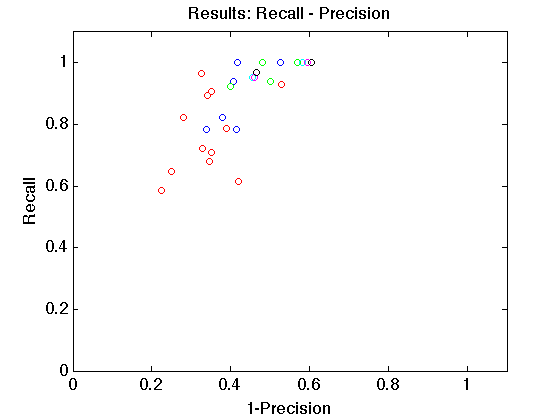
\includegraphics[scale=0.9]{files/postmethod/img/recallvsprecision2.png}
	\caption{Recall vs. 1-precision plottet fra tabel \ref{tab:postmethod_tabel2222}. Antal kombinerede resultater: 1=rød, 2=blå, 3=grøn, 4=cyan, 5=magenta, 6=sort. \label{fig:postmethod_recallprec}}
\end{figure}

% Kombinationsresultater med kommentar om metodens robusthed ved vesikelliste.
% Resultater ved "krydsprodukt" af vesiklerne.
% Begrund ifh. forord at vi kun nu ser på nye billeder da det er dem der benyttes i praksis.
% Forhåbninger om bedre resultater ved tidligere metoder (Hough, SLD). 
% Synop konkl.

\newpage
\begin{figure}[H]
  \centering
  \subfloat[47 / 23 / 18]{\label{fig:gull111}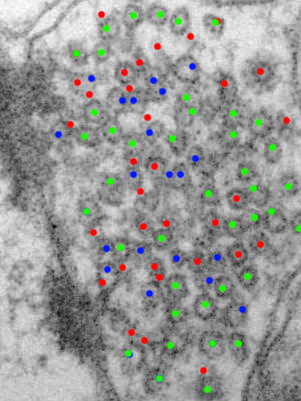
\includegraphics[width=0.26\textwidth]{files/postmethod/img/eval_1-1.png}}        
  \hspace{0.1cm}
  \subfloat[38 / 11 / 27]{\label{fig:tiger111}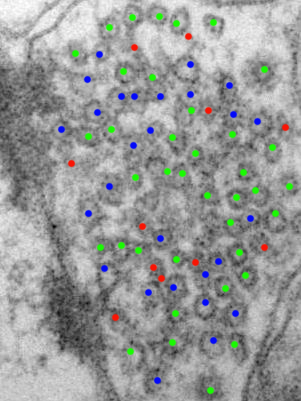
\includegraphics[width=0.26\textwidth]{files/postmethod/img/eval_1-2.png}}
  \hspace{0.1cm}
  \subfloat[40 / 29 / 25]{\label{fig:mouse111}\includegraphics[width=0.26\textwidth]{files/postmethod/img/eval_1-3.png}}\\
  \subfloat[46 / 25 / 19]{\label{fig:gull222}\includegraphics[width=0.26\textwidth]{files/postmethod/img/eval_1-4.png}}        
  \hspace{0.1cm}
  \subfloat[59 / 32 / 6]{\label{fig:tiger222}\includegraphics[width=0.26\textwidth]{files/postmethod/img/eval_1-5.png}}
  \hspace{0.1cm}
  \subfloat[42 / 14 / 23]{\label{fig:mouse222}\includegraphics[width=0.26\textwidth]{files/postmethod/img/eval_1-6.png}}
  \caption{Resultater af segmenteringen efter afstandsmåling med 6 vesikler. (a)-(f) er udført på samme celle. Under hvert billede er angivet antallet af Sand positiv (Grøn) / Falsk positiv (Rød) / Falsk negativ (Blå).}
  \label{fig:animalsss}
\end{figure}

\begin{figure}[H]
  \centering
  \subfloat[26 / 29 / 2]{\label{fig:gull4}\includegraphics[width=0.26\textwidth]{files/postmethod/img/eval_2-1.png}}        
  \hspace{0.1cm}
  \subfloat[22 / 14 / 6]{\label{fig:tiger5}\includegraphics[width=0.26\textwidth]{files/postmethod/img/eval_2-2.png}}
  \hspace{0.1cm}
  \subfloat[23 / 9 / 5]{\label{fig:mouse6}\includegraphics[width=0.26\textwidth]{files/postmethod/img/eval_2-3.png}}\\
  \subfloat[19 / 10 / 9]{\label{fig:gull7}\includegraphics[width=0.26\textwidth]{files/postmethod/img/eval_2-4.png}}        
  \hspace{0.1cm}
  \subfloat[25 / 13 / 3]{\label{fig:tiger8}\includegraphics[width=0.26\textwidth]{files/postmethod/img/eval_2-5.png}}
  \hspace{0.1cm}
  \subfloat[27 / 13 / 1]{\label{fig:mouse9}\includegraphics[width=0.26\textwidth]{files/postmethod/img/eval_2-6.png}}
  \caption{Resultater af segmenteringen efter afstandsmåling med 6 vesikler. (a)-(f) er udført på samme celle. Under hvert billede er angivet antallet af Sand positiv (Grøn) / Falsk positiv (Rød) / Falsk negativ (Blå).}
  \label{fig:animalssssssssssss}
\end{figure}
